\section{}

A ping-pong buffer is a double buffer that can be used to overlap I/O operations
with data processing to speed up a device.  The idea is that the first buffer
holds some old, but complete data which the reader can access, while the other
buffer holds some partial, incomplete but newer data which the writer is writing
to. When the writer is finished, the buffers switch and "ping-pong", so that the
reader is now reading from the second buffer, and the writer is writing to the
first buffer. This process repeats itself.
An illustration from the notes is below:

\begin{figure}[h]
  \includegraphics[page=17, width=\textwidth]{../../notes/Ch11_W20_Flow_Control.pdf}
\end{figure}

  The advantage of a ping-pong buffer is that the reader and the writer can
  access data stored in their respective buffers in any arbitrary order,
  as opposed to a FIFO buffer for example, which requires that the data is read
  in the same order as it was written in. 

  For example, if an application was doing matrix operations, the elements of a
  matrix could be written column-by-column, while the reader could read the
  matrix row-by-row.

  Another example application where a ping-pong buffer may be useful is in
  streaming video. The data in one buffer can be sent to a graphics card to
  display the video to the user, while at the same time, another buffer is being
  written to by the network card, where the video stream is coming from.
